\documentclass{article}
\usepackage[utf8]{inputenc}

\title{CS 598 SM HW1}
\author{Daniel Campos}
\date{September 23rd,2020}

\usepackage{natbib}
\usepackage{graphicx}

\begin{document}

\maketitle
\section{Chebfun Approximation $x * sin(6x)$}
\subsection{$[-\pi, \pi]$ }
As you can see in \ref{fig:-pi2pi} the functions almost match perfectly. There are minor differences in some local maximas and minimas but for the most part agree heavily
\begin{figure}[h!]
\centering
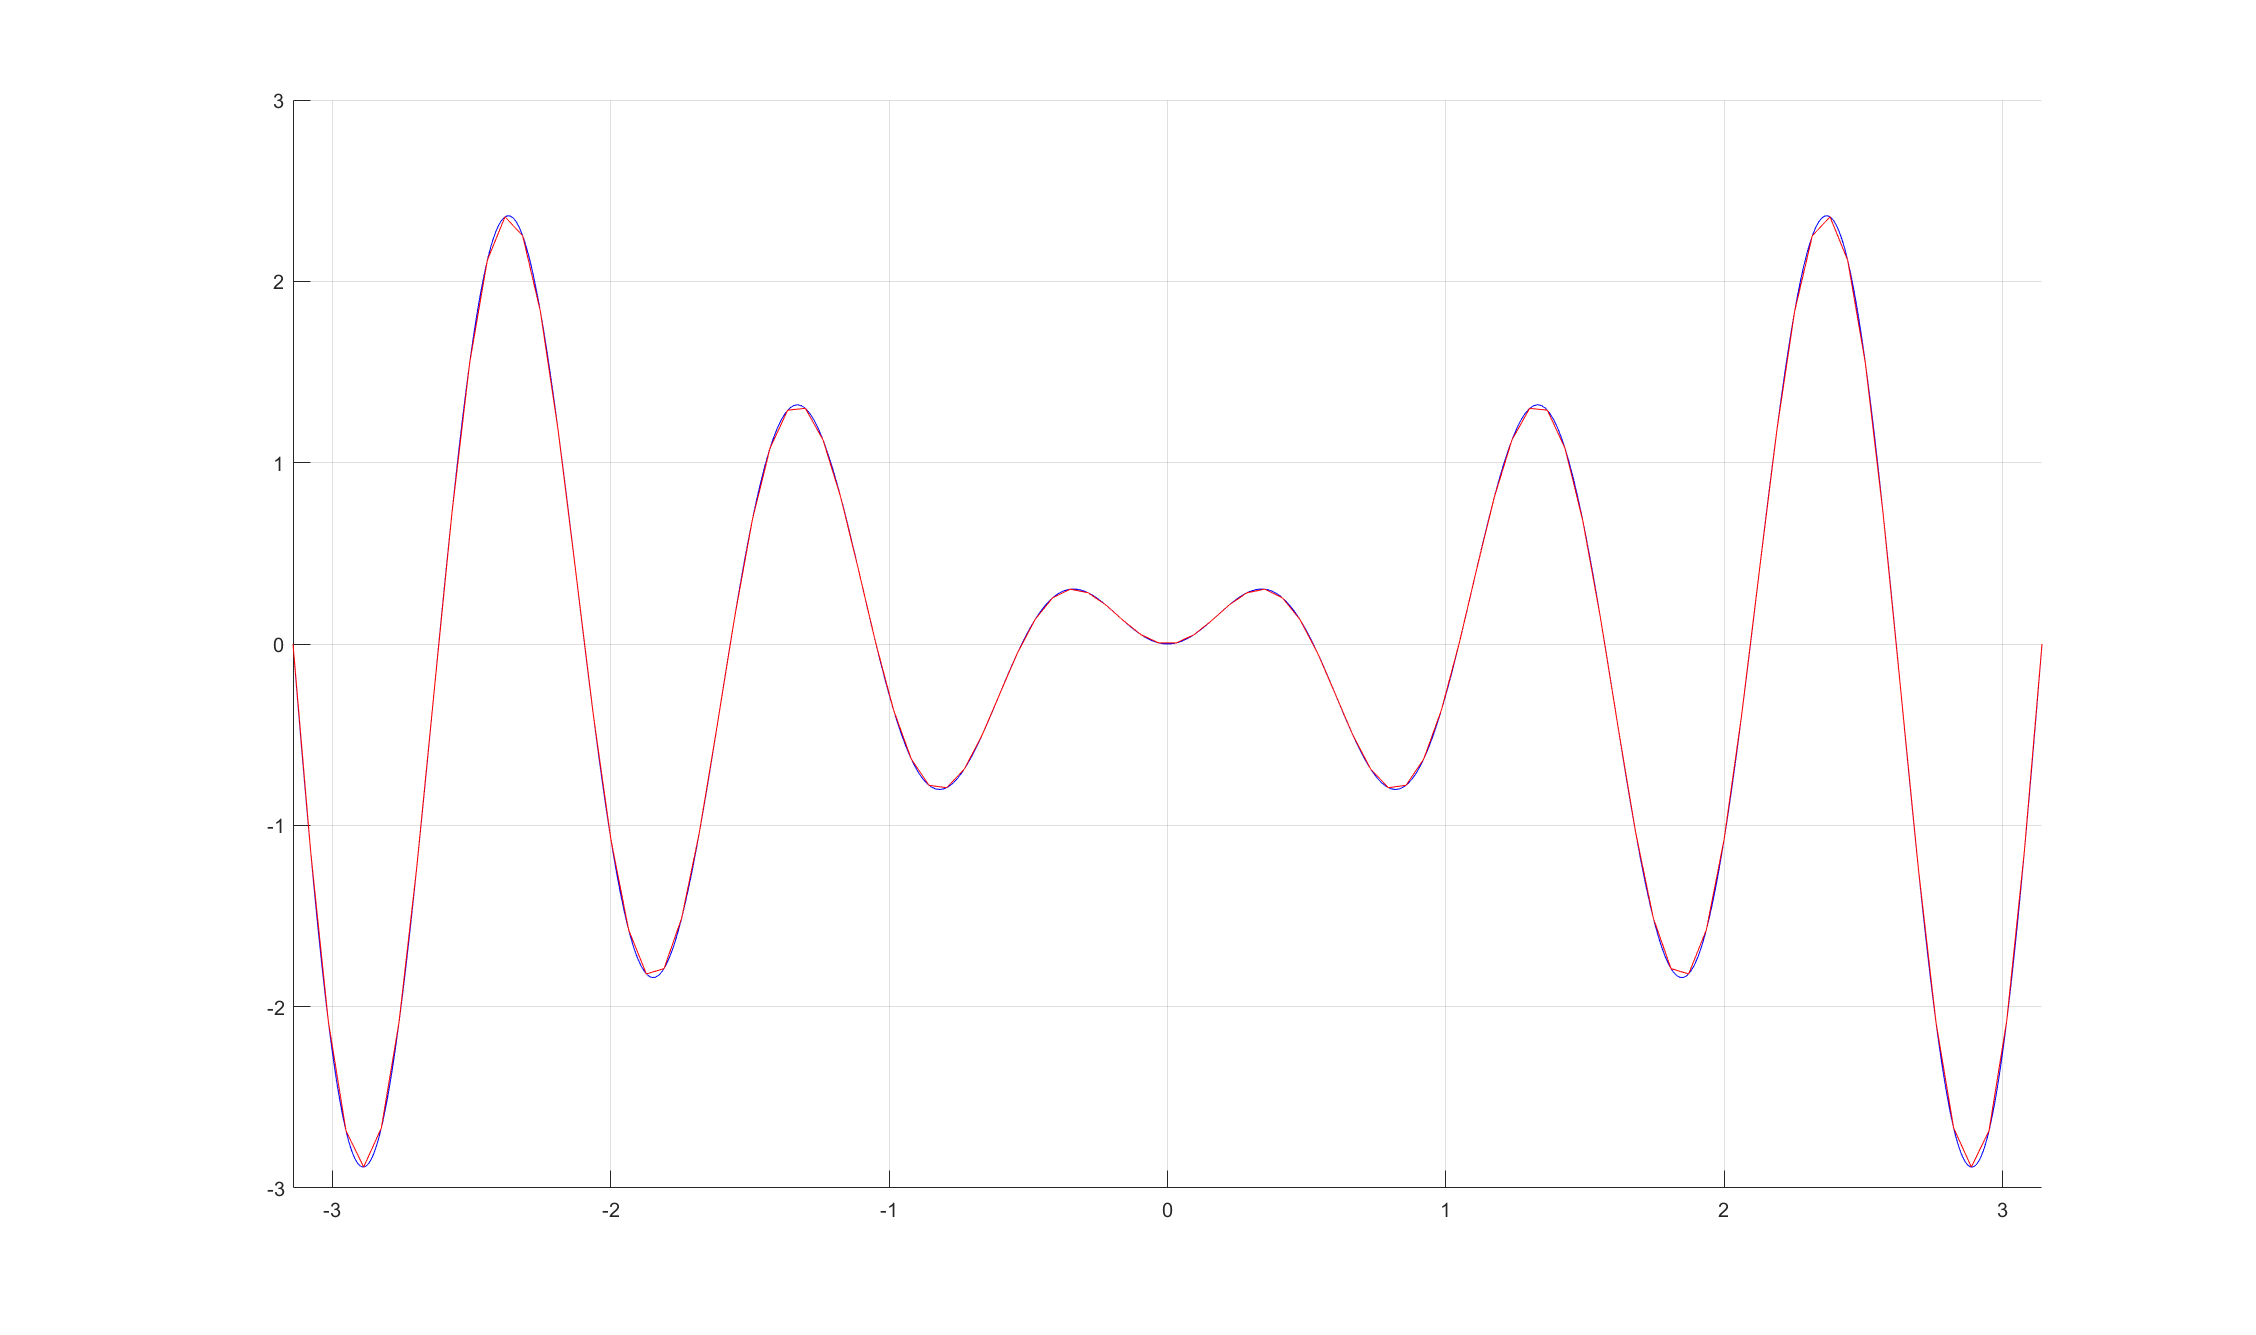
\includegraphics[scale=.2]{-pi2pi.png}
\caption{Function scaled $[-\pi, \pi]$ Red is original function, blue is chebfun}
\label{fig:-pi2pi}
\end{figure}
\subsection{$[-2\pi, 2\pi]$}
As we scale the plot to $-2\pi to 2\pi$ we can start to see how the approximation is becoming less accurate at the extremes. 
\begin{figure}[h!]
\centering
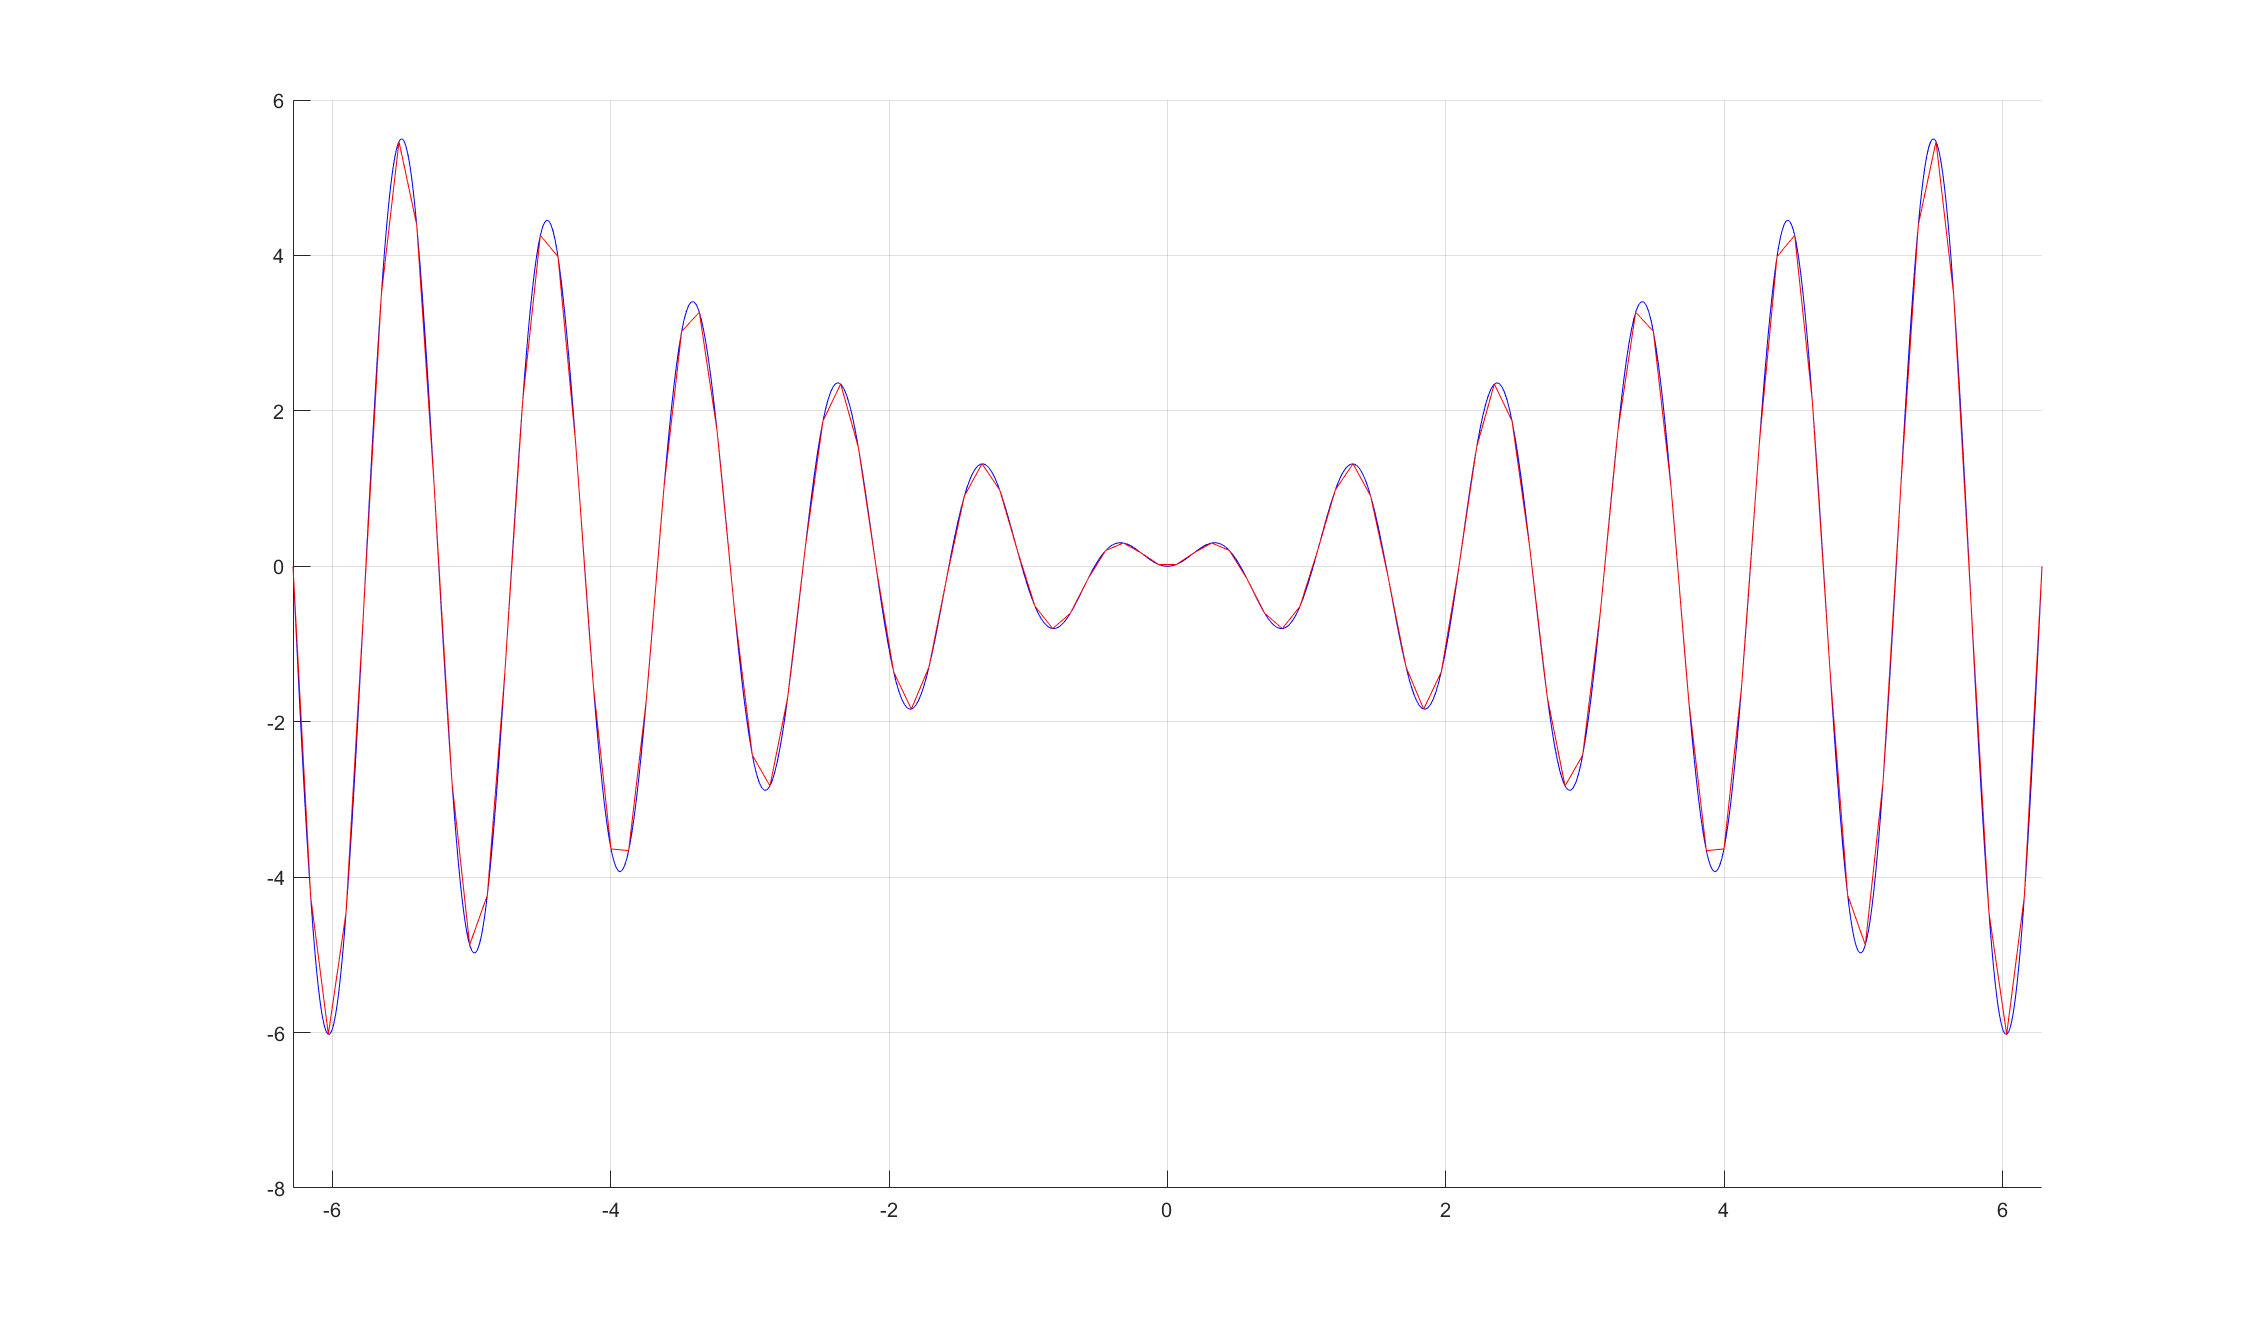
\includegraphics[scale=.2]{-2pi22pi.png}
\caption{Function scaled $[-2\pi, 2\pi]$ Red is original function, blue is chebfun}
\label{fig:-pi2pi}
\end{figure}
\subsection{Approximation error on range $[-\pi, \pi]$ }
Looking at the approximation error we can see the trend we mention in the previous subsection where error increases the further we travel from 0.
\begin{figure}[h!]
\centering
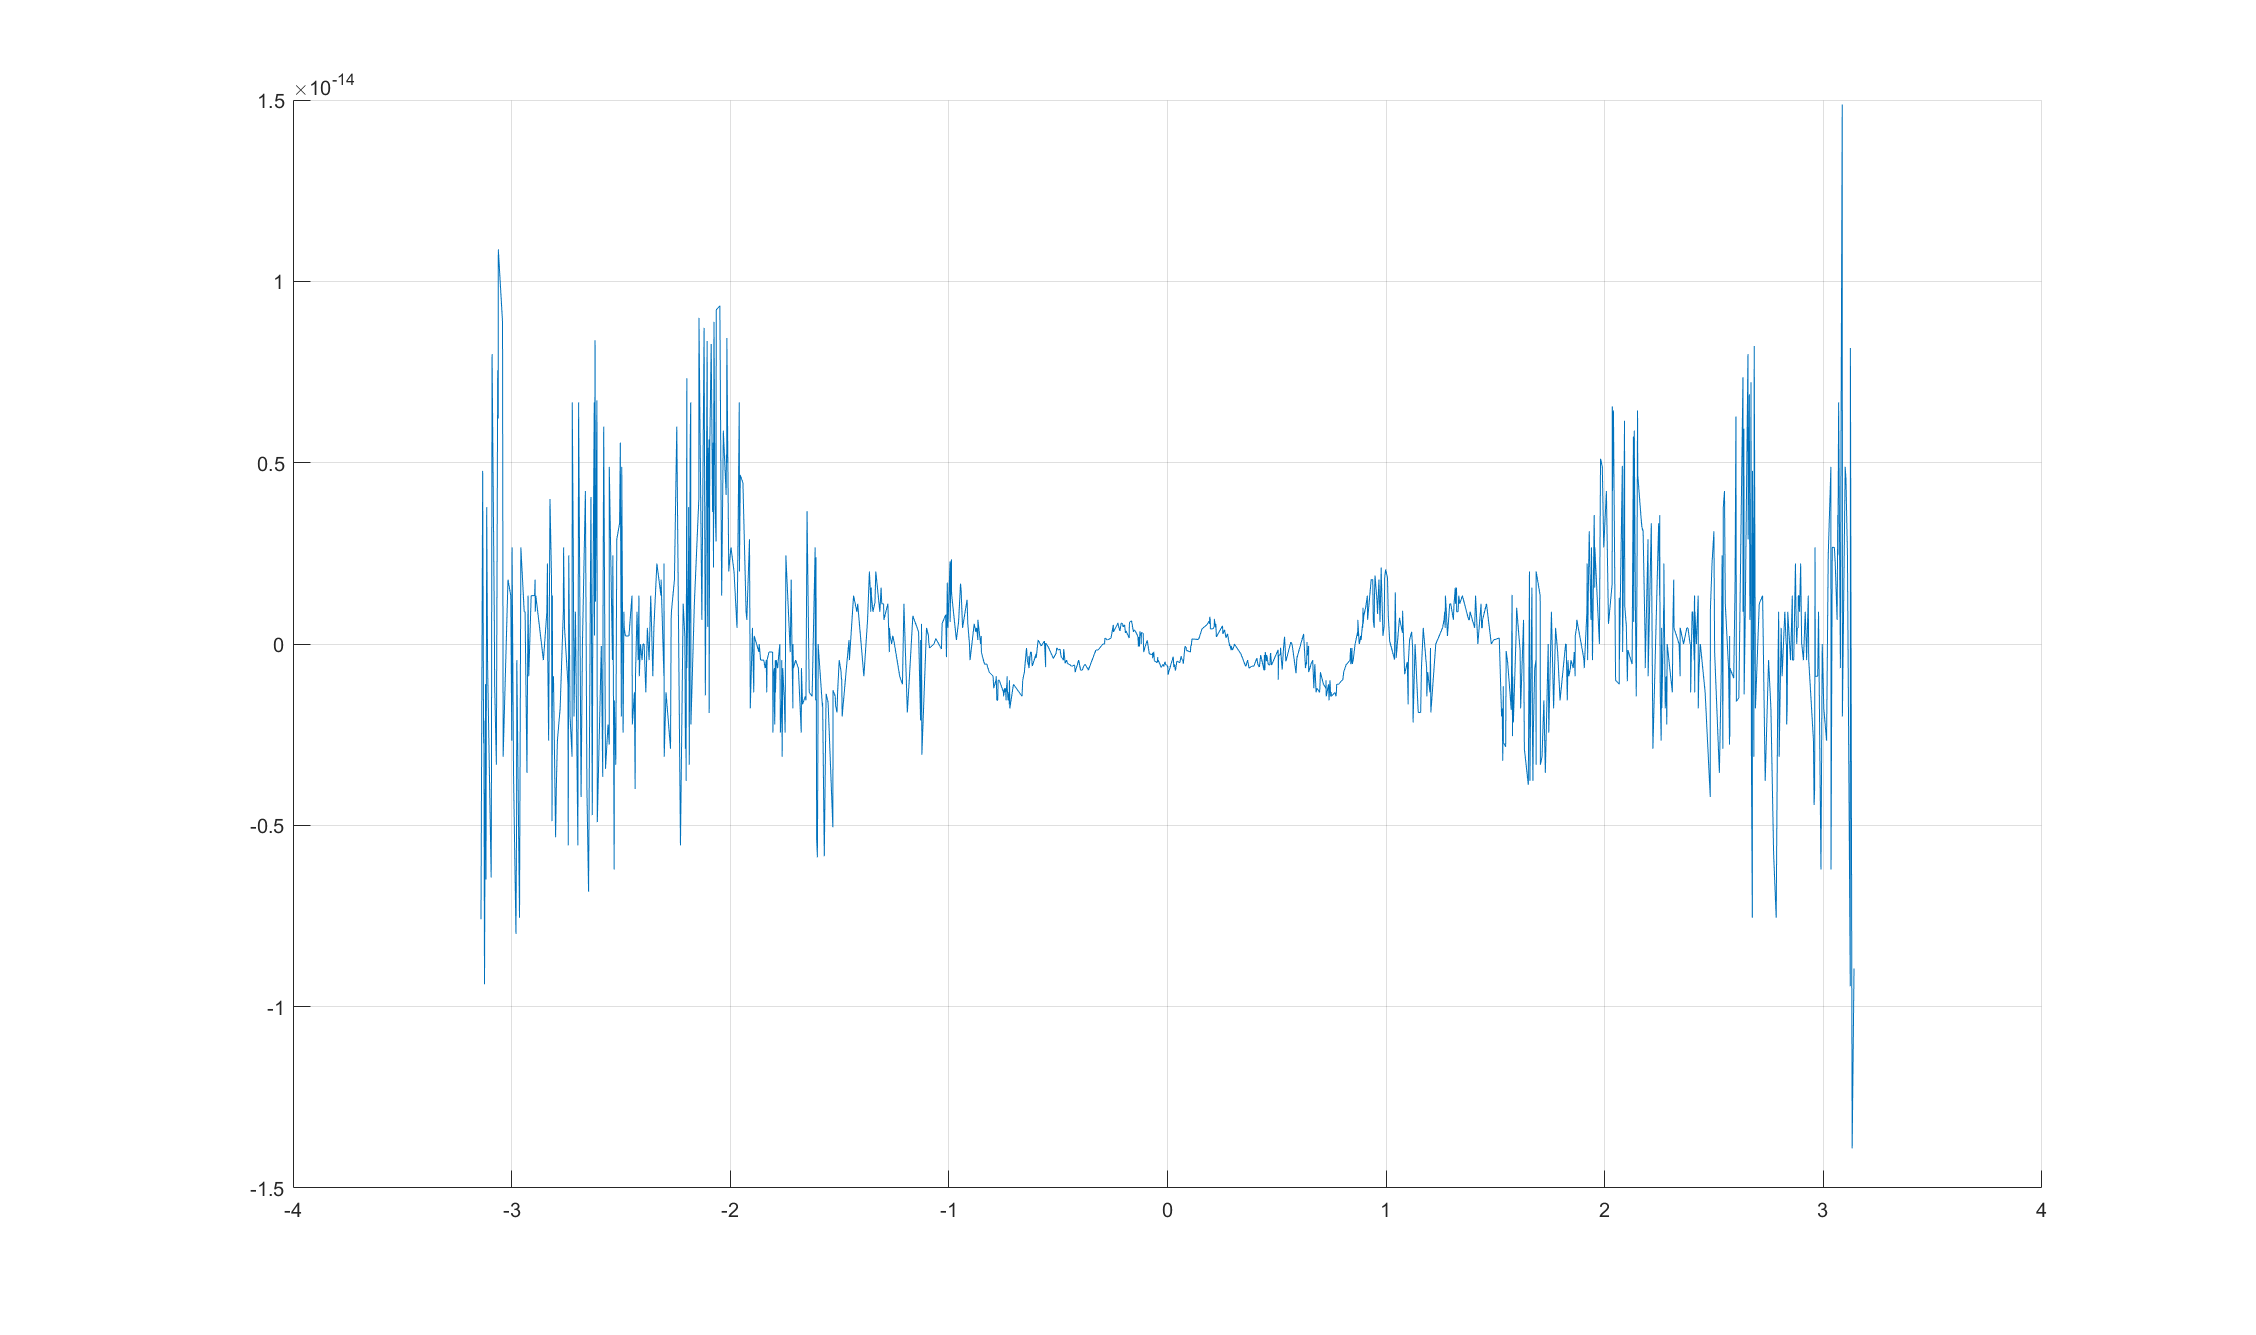
\includegraphics[scale=.2]{approxerror.png}
\caption{Approximation error  $[-\pi, \pi]$ Y axis is absolute error, X axis is function input}
\label{fig:approxerror}
\end{figure}

\section{Noisy Functions $tanh(8(x-.5)) + 10^-6*noise$}
Replace tanh with sigmoid.
\subsection{$f(x) $}
When we replace tanh with sigmoid we see similar behavior in the first equation f(x) but can approximate the equation with a lower eps value.. As show in in \ref{fig:-3f} we are able to approximate most of the function with a low eps of 1e-3 and fully match the function with an eps of 1e-9 \ref{fig:-9f}. Moreover, unlike the original f(x), our sigmoid f(x) is able to converge even without the use of eps. 
\begin{figure}[h!]
\centering
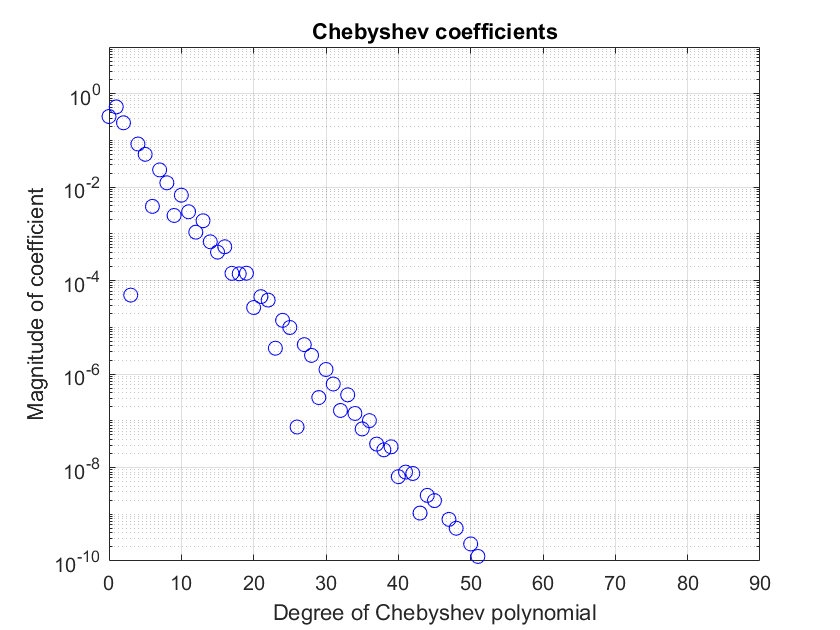
\includegraphics[scale=.5]{fnone.png}
\caption{No eps}
\label{fig:fnone}
\end{figure}

\begin{figure}[h]
\centering
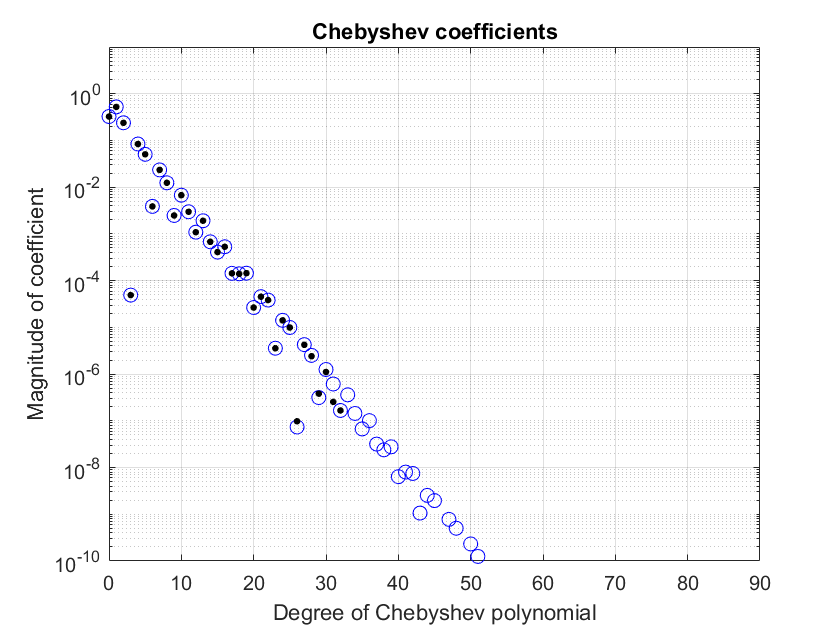
\includegraphics[scale=.5]{-3f.png}
\caption{eps 1e-3}
\label{fig:-3f}
\end{figure}

\begin{figure}[h!]
\centering
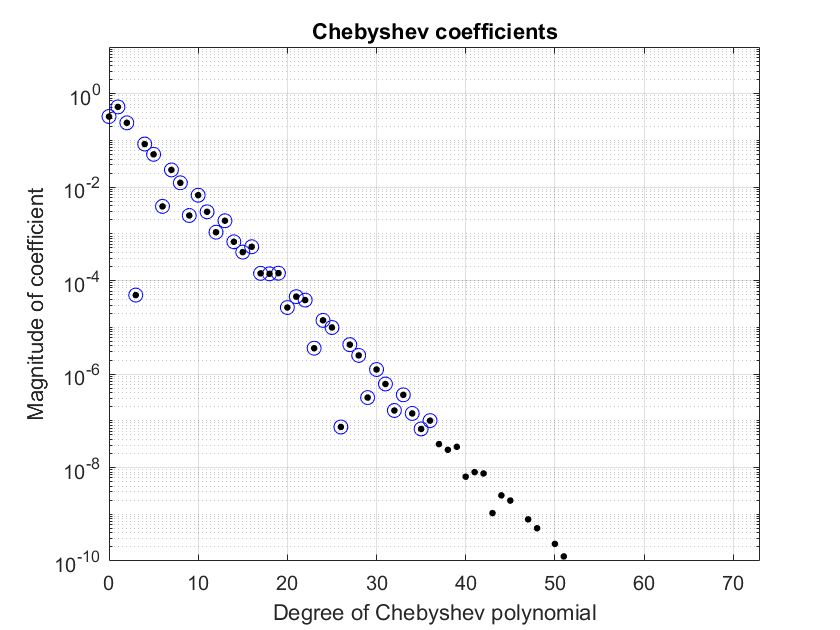
\includegraphics[scale=.5]{-6f.png}
\caption{eps 1e-6}
\label{fig:-6f}
\end{figure}

\begin{figure}[h!]
\centering
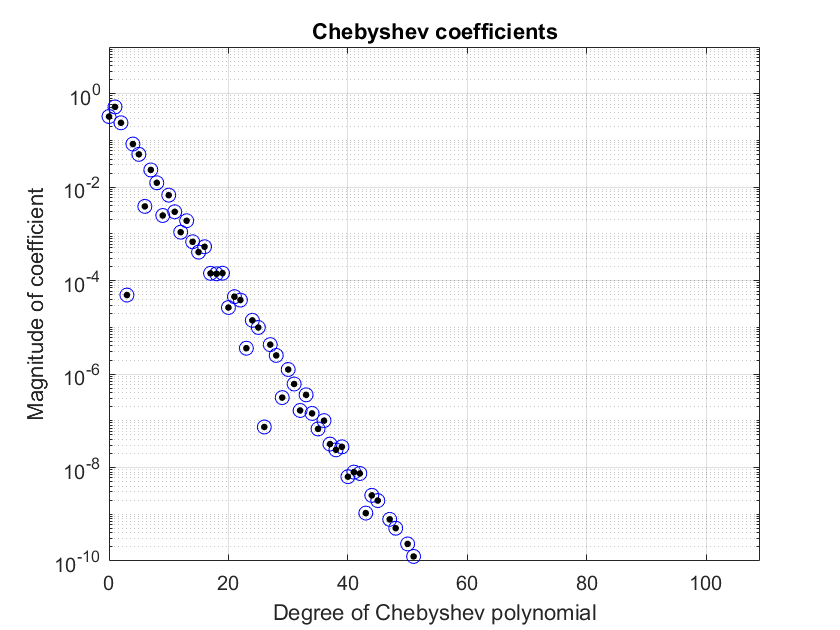
\includegraphics[scale=0.5]{-9f.png}
\caption{eps 1e-9}
\label{fig:-9f}
\end{figure}

\begin{figure}[h!]
\centering
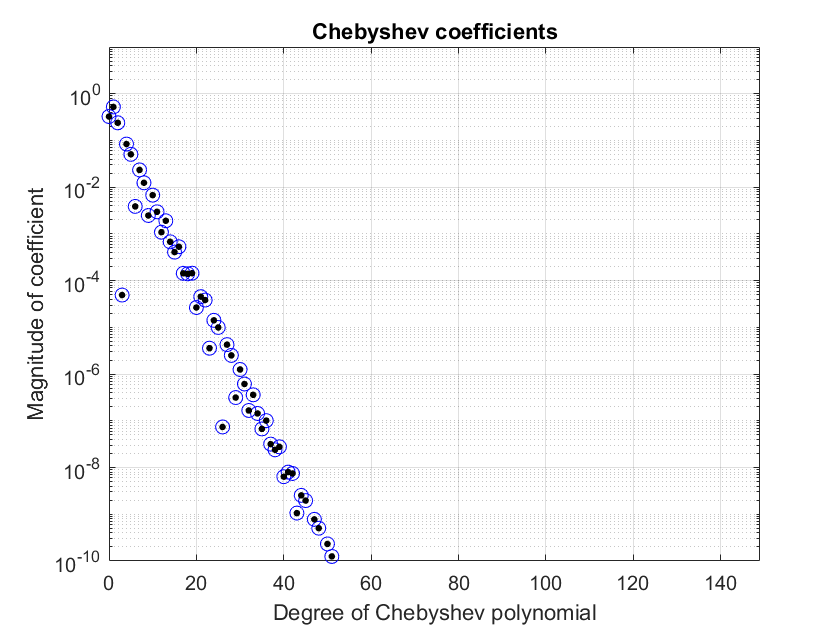
\includegraphics[scale=.5]{-12f.png}
\caption{eps 1e-12}
\label{fig:-12f}
\end{figure}

\subsection{$g(x) $}
For g(x) the use of sigmoid behaves much more like the example. With any eps of 1e-3 \ref{fig:-3g} we are unable to capture much of the original function. As we scale the eps we start to capture more of the original function but completely miss the steep drop off around 300 degrees \ref{fig:-9g}. When we scale to 1e-12 we are finally able to capture the drop off in the noisy function in an accurate way. 
\begin{figure}[h!]
\centering
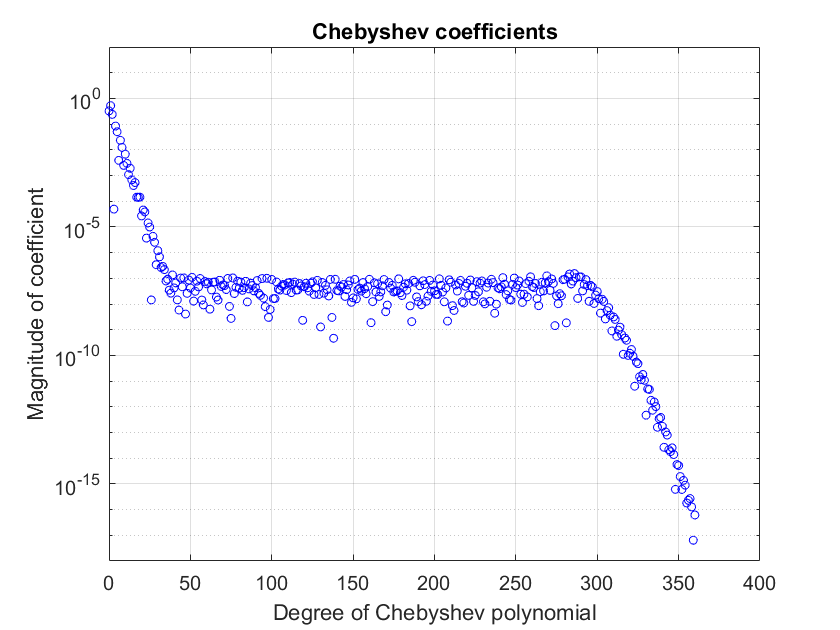
\includegraphics[scale=.5]{gnone.png}
\caption{No Eps}
\label{fig:gnone}
\end{figure}
\begin{figure}[h!]
\centering
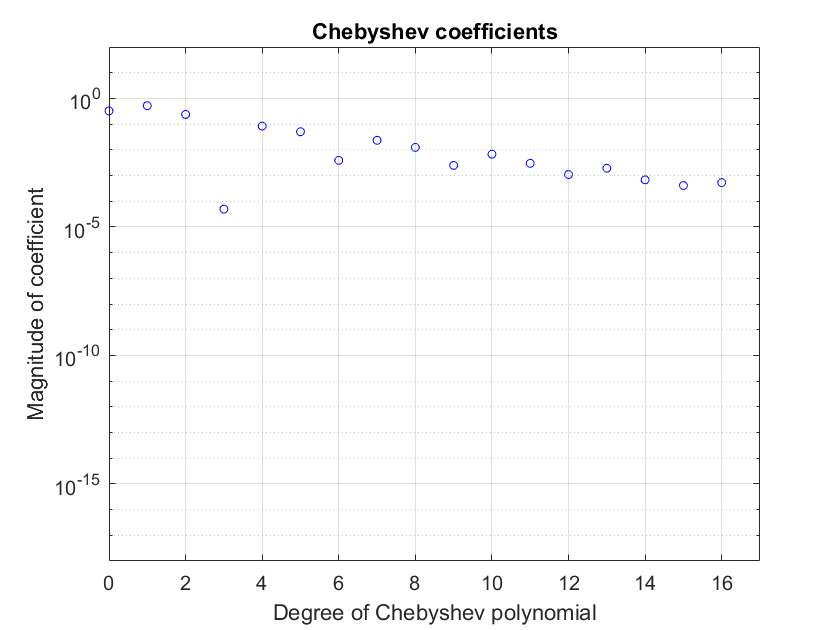
\includegraphics[scale=.5]{-3g.png}
\caption{eps 1e-3}
\label{fig:-3g}
\end{figure}
\begin{figure}[h!]
\centering
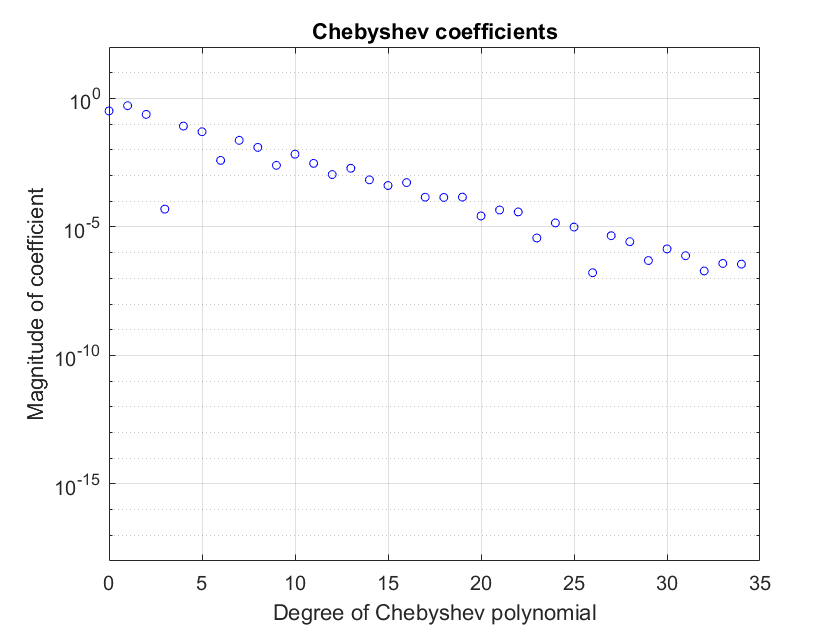
\includegraphics[scale=.5]{-6g.png}
\caption{eps 1e-6}
\label{fig:-6g}
\end{figure}
\begin{figure}[h!]
\centering
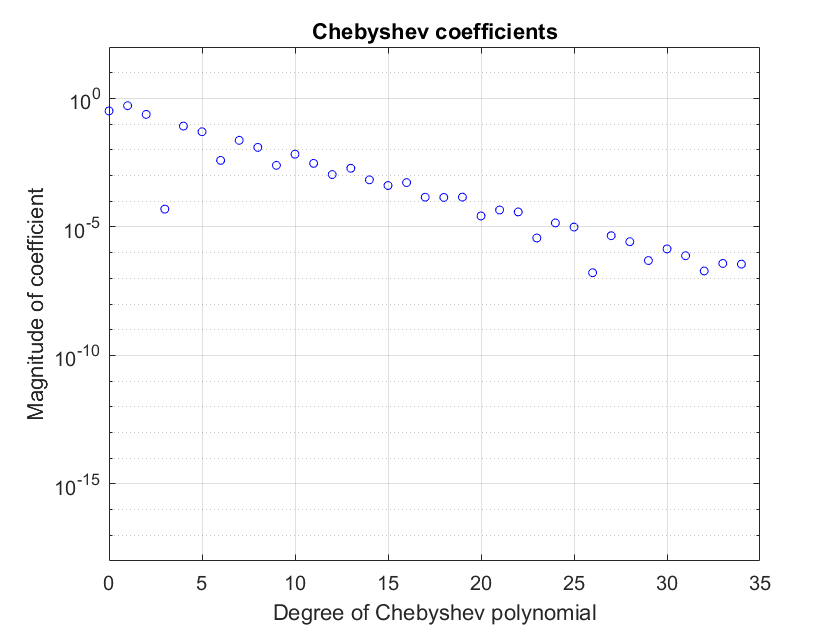
\includegraphics[scale=.5]{-9g.png}
\caption{eps 1e-9}
\label{fig:-9g}
\end{figure}
\begin{figure}[h!]
\centering
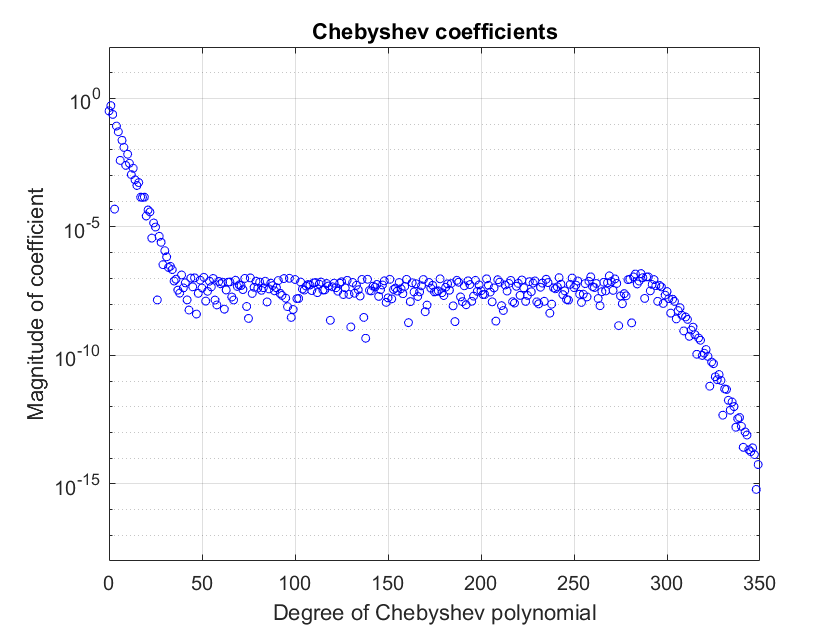
\includegraphics[scale=.5]{-12g.png}
\caption{eps 1e-12}
\label{fig:-12g}
\end{figure}
\section{Discussion}
This framework can be used to approximate numerical functions that can be expensive and approximation works well like a log function. Since most of these functions tend to saturate and the cost of computing the full values can be very expensive especially if we only need to understand the curve. Obviously just like anything that can have a fractal nature the closer we look(more sample points on the curve) the greater the error will be. \\
We can expect to have problems where the noise introduced is either quite jagged or the nature of the function does not matched the curved shape as Polynomial interpolation(which Chebyshev points are used for) is useful for dense curved data. If we are looking at some kind of data that only has a curve with some type of higher dimension transformation(like much of the data used for machine learning) Chebyshev point are likely to produce bad approximations.
\end{document}
